\section{The Terrain}
The terrain that the hiker walks on is randomly generated for every game. It is represented by 2D-Splines and is approximated by polylines for collision detection and rendering.

\subsection{Structure}

Internally, the terrain consists of a list of biomes. 
Each biome in turn consists of a list of points $(p_0, p_2, \dots, p_n)$. 
For a reasonably smooth terrain, we decided to use 2D $C^1$-continuous Hermite-Splines to interpolate in between the points. 
Here, every spline interpolates between a start $p_i = (x_i, y_i)^T$ and end point $p_{i+1} = (x_{i+1}, y_{i+1})^T$ given in 2D space. 
To do this, we use separate 1D $C^1$-continuous hermite splines $H_x(t), H_y(t)$ for $x$- and $y$-direction that are both dependent on an artificial third prameter $t$.
This parameter $t$ is roughly equivalent to the distance along the terrain. 
Therefore, it is set to $t_0 = 0$ for the first point and calculated using euclidian distance for every further point.

To get the position of the terrain at a given $t$ we combine the two spline evaluations into a point $(H_x(t), H_y(t))^T$.
We calculate the $C^1$-continuous Hermite-Spline $H_{i,x}(t)$ between a given start and end point $x_{i}, x_{i+1}$ using start and end derivatives $dx_{i}, dx_{i+1}$ and a start value $t_i$ for $t$ as follows. The procedure is analogous for $H_{i,y}(t)$.

% For given start and end points ($(x_s, y_s), (x_e, y_e)$), a given start $t_s$ and given start and end derivatives $(dx_s, dy_s), (dx_e, dy_e)$, we calculate the appropriate splines $H_x(t), H_y(t)$ in the following way:\\
\begin{align}
  t_{i+1} = & t_{i} + \sqrt{(x_{i+1} - x_{i})^2 + (y_{i+1} - y_{i})^2} \\
  H_{i,x}(t) = & (1- 3t^2 + 2t^3)x_{i} + (3t^2 - 2t^3)x_{i+1} \notag\\
  & + (t-2t^2 + t^3)(x_{i+1}-x_{i})dx_{i} \notag\\
  & + (t^3 - t^2)(x_{i+1}-x_{i})dx_{i+1} 
\end{align}

We also experimented with $C^2$-continuous splines. 
In contrast to our method, here the first derivatives at the start and end of a spline are determined by conditions for the second order derivatives and do not need to be provided.
However, these splines typically require us to know all interpolated points at once. 
Consequently, this approach is unsuitable for our generation that is performed in an online manner.
For this reason, we chose to stick with $C^1$-continuous splines and provide the first order derivatives. 

These first order derivatives can be freely chosen but need to match at the borders between splines since the splines are $C^1$-continuous.
Therefore, we provided the start derivative $(dx_0, dy_0)^T = (1, 0)^T$ that corresponds to even terrain. 
From there, we set the derivative of the end of a spline piece to the slope for piecewise linear interpolation:
\begin{align}
  & \forall i\in\{0,1, \dots, n-1\}: \notag\\
  & \quad (dx_{i+1}, dy_{i+1}) = (x_{i+1} - x_i, y_{i+1} - y_i)
\end{align}

The individual spline pieces $H_i(t) = (H_{i, x}(t), H_{i, y}(t))^T$ are then combined into one continuous function $H(t)$, that allows us to interpolate the terrain at any $t$-value between the first and last point.
Using this method, we can generate a spline-based interpolation of the ground points in an online setting which we need for the terrain generation.
%This is particularly useful for the generation of the terrain, where the points are generated iteratively using the existing spline representation.

A good overview over hermite splines is given in \cite{NumerischeGrundlagen2024}.

\subsection{Generation}

At the start of the game, the terrain is generated with one start biome of fixed length. After that, a new biome of the same fixed length is generated whenever the hiker gets close to the right border of the currently generated terrain. 
This is done concurrently to not disturb the playing experience.
Similarly, whenever a biome is no longer visible it is removed from the terrain.

The basepoints used to specify the ground of each biome are generated in an iterative manner.
The overall form of the ground in a biome is specified by the terrain phases $ph_1, ph_2, \dots, ph_n$ of this biome as well as a special starting terrain phase $ph_{s}$ that determines the first few point of the ground.
Here, each terrain phase has the following format: 
\begin{align}
  ph = (\delta v, r, m)
\end{align}
Here, $\delta v \in\R^2$ is the average vector to be added to the last point to generate the next one, $r \in [0,1)$ is the randomness, limiting how much we can rotate the average vector, and $m \in \N$ is the number of points to be generated using this phase before selecting a new phase.

To generate a new point $p_{i+1}$ using the existing terrain up to point $p_i$ and a terrain phase $ph = (\delta v, r, m)$, we first determine the \hyperref[angleRange]{angular range} $[min, max]$ in which generation of a new point is allowed using alg. \ref{alg:maxAngleCalc} for $max$ and its analogon for $min$.
Then, we generate a new point by adding $\delta v$ rotated to a random angle in the range $[min , max]$. 
If the angular range $[min, max]$ is empty, no such point can be generated. 
Therefore, we need to \hyperref[retracing]{retrace} some of the already generated points and try to generate the terrain starting from an earlier point.
%The procedure for generation a new point is described in \hyperref[alg:genNextPoint]{Algorithm \ref{alg:genNextPoint}}.

%{
%
%  \centering
%  \begin{figure}[h]
%  % \begin{minipage}{0.485\textwidth}
%    \vspace{-\abovedisplayskip}
%    \begin{algorithm}[H]
%    \caption{Generating a new point}\label{alg:genNextPoint}
%    \hspace*{\algorithmicindent} \textbf{Input:} $ph = (\delta v, r, m)\in\R^2\times[0,1)\times \N, \, $\\
%    \hspace*{\algorithmicindent} \hphantom{\textbf{Input:}} $p_i\in\R^2, \, terrain\in\left(\R^2\right)^n$\\
%    \hspace*{\algorithmicindent} \textbf{Output:} $p_{i+1}\in \{\bot\}\cup \R^2$
%      \begin{algorithmic}[1]
%      \Procedure{GenerateNextPoint}{$ph, p_i, terrain$}
%      \State $min_a \gets$ \Call{CalculateMinAngle}{$ph, p_i, terrain$}
%      \State $max_a \gets$ \Call{CalculateMaxAngle}{$ph, p_i, terrain$}
%      \If{$min_a = \bot \lor max_a = \bot$}
%        \State \Return $\bot$
%      \EndIf
%      \State $p_{i+1} \gets p_i + $ \Call{RotateRandom}{$\delta v, min_a, max_a$}
%      \State \algorithmiccomment{rotate $\delta v$ by random angle in $[min_a, max_a]$}
%      \State \Return $p_{i+1}$
%      \EndProcedure
%      \end{algorithmic}
%    \end{algorithm}
%  %\end{minipage}
%  \end{figure}
%}
%\vspace{\belowdisplayskip}

{
  \centering
  %\begin{minipage}{0.485\textwidth}
  \begin{figure}[h]
    \vspace{-\abovedisplayskip}
    \begin{algorithm}[H]
    \caption{Calculating the maximum angle}\label{alg:maxAngleCalc}
    \hspace*{\algorithmicindent} \textbf{Input:} $ph = (\delta v, r, m)\in\R^2\times[0,1)\times \N, \, $\\
    \hspace*{\algorithmicindent} \hphantom{\textbf{Input:}} $p_i\in\R^2, \, terrain\in\left(\R^2\right)^n$\\
    \hspace*{\algorithmicindent} \textbf{Output:} $\alpha\in \{\bot\}\cup[-\pi r, \pi r)$
      \begin{algorithmic}[1]
      \Procedure{CalculateMaxAngle}{$ph, p_i, terrain$}
      \State $c_{max} \gets 30; \quad \delta\alpha_{min} \gets 0.01$
      \State $\alpha_{min} \gets -\pi r; \quad \alpha_{max} \gets \pi r$
      \State $\delta\alpha \gets \alpha_{max}; \quad \alpha \gets \alpha_{max}; \quad c \gets 0$
      \While{$(c < c_{max} \land \delta\alpha > \delta\alpha_{min}\land \alpha \leq \alpha_{max})$}
      \State $next\gets p_i + $\Call{Rotate}{$\delta v, \alpha$}
      \If{\Call{FulfillsConstraints}{$p_i, next, terrain$}}
        \State $\delta\alpha \gets \frac{\delta\alpha}{2}$ \algorithmiccomment{lower step size}
        \State $\alpha \gets \alpha + \delta\alpha$
      \Else
        \State $\alpha \gets \alpha - \delta\alpha$ \algorithmiccomment{take back last step}
      \EndIf

      \If{$\alpha \leq \alpha_{min}$} \algorithmiccomment{No $\alpha\in(\alpha_{min}, \alpha_{max}]$ found}
        \State $\alpha \gets \alpha_{max}$
        \State $\delta\alpha \gets \frac{\delta\alpha}{2}$ \algorithmiccomment{Try again with smaller step size}
      \EndIf
      \State $c \gets c + 1$
      \EndWhile

      \State \textbf{if} $c = c_{max}$ \textbf{then} \Return $\bot$ \algorithmiccomment{No viable $\alpha$ found}
      %  \State \Return $\bot$
      %\EndIf

      \State \Return $\alpha - \delta\alpha$ \algorithmiccomment{Restore last viable $\alpha$}
      \EndProcedure
      \end{algorithmic}
    \end{algorithm}
  %\end{minipage}
  \end{figure}
}

\subsubsection{Calculating the angular range}
\label{angleRange}
The angular range in which generation is allowed is defined by a $min$ and $max$ angle which are determined using a bisection method.
% More precisely, we iteratively determine these angles by trying different angles and checking whether the terrain would fulfill the constraints if the new point was generated using the current angle and terrain phase. If so, we can try a larger angle in case of $max$ and a smaller angle in case of $min$.
% The delta angle $\delta_a$ in beween tried angles is halfed for every successful try. If $\delta_a$ gets small enough or we exceed a fixed limit of tries, we return the best previously found angle if one exists or that there is no suitable angle.
This procedure is described in detail for determining $max$ in alg. \ref{alg:maxAngleCalc}.
It is analogous for determining $min$. 
Determining $min$ and $max$ in an example case is illustrated in fig. \ref{pic:calculateAngleRange}.

\imagewithwidth{figures/CalculateAngleRange.pdf}{1.05\columnwidth}{pic:calculateAngleRange}{Calculating the range $[min, max]$ of angles in which the generation of a new point from the last point of the existing terrain and using a given terrain phase $(\delta v, r, m)$ is possible.}{}
\vspace{-\abovedisplayskip}

\subsubsection{Retracing}
\label{retracing}
Although we check all constraints for every generated point, sometimes we cannot generate a new point from the existing terrain. 
Then, we need to retrace parts of the previously generated terrain.
To do so, we remove a fixed number of points from the terrain. 
After that, the generation continues normally. Retracing is illustrated in fig. \ref{pic:retrace}.

\vspace{-\abovedisplayskip}
\imagewithwidth{figures/Retrace.pdf}{\columnwidth}{pic:retrace}{Trying to generate a new point with terrain phase $ph=(\delta v, r, m)$ when the constraints do not allow that. Results in removing of the last few generated points.}{}
\vspace{-\abovedisplayskip}
\newpage
If we cannot regenerate all points that were removed before we retrace again, then we increment how many points need to be removed by a fixed number and retrace again.
We also tried an exponentially increasing retrace count. 
However, that regularly lead to the entire ground being regenerated which took longer overall. Therefore, we decided to use the linearly increasing retrace count.

%\imagewithwidth{figures/Retrace.pdf}{\columnwidth}{pic:retrace}{Trying to generate a new point with the current terrain phase $ph=(\delta v, r, m)$ when the constraints do not allow that. Results in retracing, that is removing of the last few generated points.}{}

%Including the retracing we get the procedure in \hyperref[alg:maxAngleCalc]{Algorithm \ref{alg:genGround}} for generating the ground of a biome of specified length.

%{
%  \centering
%  \begin{figure}[h]
%  %\begin{minipage}{0.485\textwidth}
%    \vspace{-\abovedisplayskip}
%    \begin{algorithm}[H]
%    \caption{Generating the ground of a biome}\label{alg:genGround}
%    \hspace*{\algorithmicindent} \textbf{Input:} $ph_{s} = (\delta v, 0, m) \in\R^2\times\{0\}\times \N, $\\
%    \hspace*{\algorithmicindent} \hphantom{\textbf{Input:}} $phases = \{ph_1, \dots, ph_n | ph_i = $ \\
%    \hspace*{\algorithmicindent} \hphantom{\textbf{Input:}} \hphantom{$phases = \{\}$} $(\delta v_i, r_i, m_i)\in\R^2\times[0,1)\times \N\}$\\
%    %\hspace*{\algorithmicindent} \hphantom{\textbf{Input:}} $phases = \{ph_1, \dots, ph_n | ph_i = (\delta v_i, r_i, m_i)\in\R^2\times[0,1)\times \N\}$\\
%    \hspace*{\algorithmicindent} \hphantom{\textbf{Input:}} $p_0\in \R^2, length \in \R$\\
%    \hspace*{\algorithmicindent} \textbf{Output:} $ground = (p_0, p_1, \dots, p_k) \in (\R^2)^{k+1}$
%      \begin{algorithmic}[1]
%      \Procedure{GenerateGround}{$ph_{s}, phases, p_0, length$}
%      \State $ph \gets ph_{start}, p \gets p_0, t\gets t_0$
%      \State $ground \gets (p_0), phasePointCount \gets 0$
%      \While{$p_x < p_{0,x} + length$}
%        \If{$pointCount = r$} 
%          \State \algorithmiccomment{All points of current phase generated}
%          \State $ph \gets$ \Call{RandomPhase}{$phases$}
%          \State $phasePointCount = 0$
%        \EndIf
%        \State $terrain \gets$ \Call{CalculateTerrain}{$ground$}
%        \State \Comment{\parbox[t]{.8\linewidth}{Terrain within fixed range of last point in $ground$. Needed to check all constraints.}}
%        \vspace{.1cm}
%        \State $p_{new} \gets$ \Call{GenerateNewPoint}{$ph, p, terrain$}
%        \If{$p_{new} = \bot$} \Comment{Can't generate next point}
%          \State \Call{Retrace}{$ground$}
%        \Else
%          \State $ground.add(p_{new})$
%          \State $p \gets p_{new}$
%        \EndIf
%      \EndWhile
%      \State \Return $ground$
%      \EndProcedure
%      \end{algorithmic}
%    \end{algorithm}
%  %\end{minipage}
%\end{figure}
%}

\subsection{Contraints}
\label{constraints}
To determine the angular range for generation and to verify that the newly generated point is appropriate, we formulate several constraints on the terrain.
These constraints ensure that the terrain does not intersect with itself, that there are no too thin parts in the terrain, that it is navigatable by the hiker, and does not generate backwards.
The problems that would arise in the terrain generation should these constraints be violated can be seen in fig. \ref{fig:constraints}.

\begin{figure}[htbp]
  \centering
  \begin{subfigure}{.5\linewidth}
    \centering
    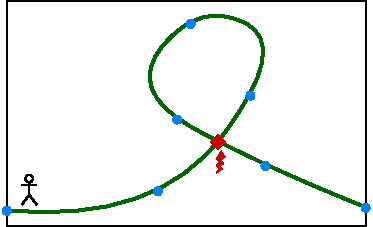
\includegraphics[width=.97\linewidth]{figures/constraints/NoSelfPenetration.pdf}
    \caption{No Selfpenetration}
    \label{pic:noSelfPenetration}
  \end{subfigure}%
  \begin{subfigure}{.5\linewidth}
    \centering
    \includegraphics[width=.97\linewidth]{figures/constraints/minimalBasepointDistance.pdf}
    \caption{Minimal Basepoint Distance}
    \label{pic:minimalBasepointDistance}
  \end{subfigure}

  \vspace{.5cm}
  \begin{subfigure}{.5\linewidth}
    \centering
    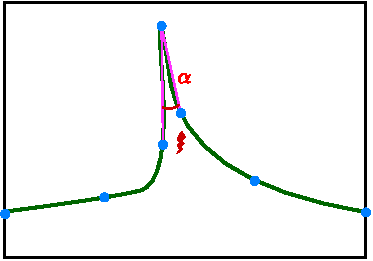
\includegraphics[width=.97\linewidth]{figures/constraints/MinimalBasepointAngle.pdf}
    \caption{Minimal Basepoint Angle}
    \label{pic:minimalBasepointAngle}
  \end{subfigure}%
  \begin{subfigure}{.5\linewidth}
    \centering
    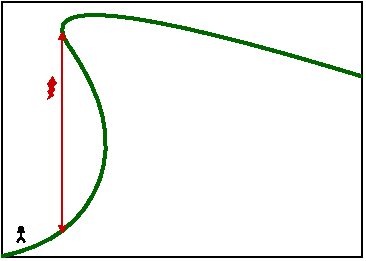
\includegraphics[width=.948\linewidth]{figures/constraints/TerrainJumpeable.pdf}
    \caption{Terrain Jumpable}
    \label{pic:terrainJumpeable}
  \end{subfigure}

  \vspace{.5cm}
  \begin{subfigure}{.5\linewidth}
    \centering
    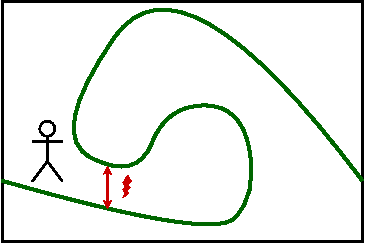
\includegraphics[width=.948\linewidth]{figures/constraints/HikerClearanceHeight.pdf}
    \caption{Hiker Clearance (Height)}
    \label{pic:hikerClearanceHeight}
  \end{subfigure}%
  \begin{subfigure}{.5\linewidth}
    \centering
    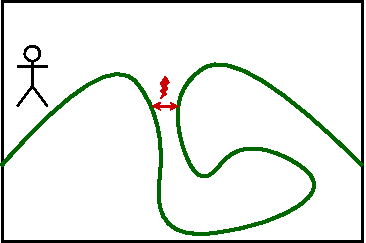
\includegraphics[width=.948\linewidth]{figures/constraints/HikerClearanceWidth.pdf}
    \caption{Hiker Clearance (Width)}
    \label{pic:hikerClearanceWidth}
  \end{subfigure}

  \vspace{.5cm}
  \begin{subfigure}{.5\linewidth}
    \centering
    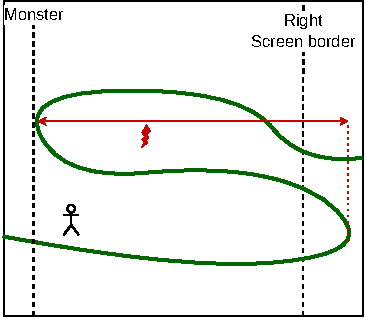
\includegraphics[width=.948\linewidth]{figures/constraints/MaximalOverhangWidth.pdf}
    \caption{Maximal Overhang Width}
    \label{pic:maximalOverhangWidth}
  \end{subfigure}%
  \begin{subfigure}{.5\linewidth}
    \centering
    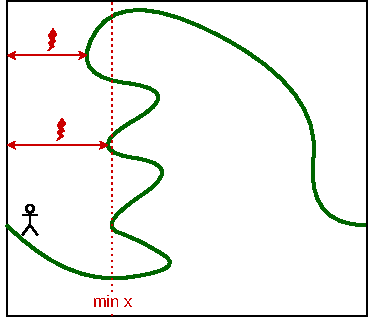
\includegraphics[width=.96\linewidth]{figures/constraints/MinimalXPos.pdf}
    \caption{Minimal x-Pos}
    \label{pic:minimalXPos}
  \end{subfigure}

  \vspace{.3cm}
  \begin{subfigure}{\linewidth}
    \centering
    
\includegraphics[width=\linewidth]{figures/constraints/Legend.pdf}
    %\caption{Legend}
    \label{pic:constraintsLegend}
  \end{subfigure}
  \vspace{-3\abovedisplayskip}
  \caption{Examples of terrains that could be generated if the constraints are ignored.}
  \label{fig:constraints}
  \vspace{-\abovedisplayskip}
\end{figure}
\vspace{-\abovedisplayskip}

%\newpage
\subsection{Representation}

For both rendering and collision detection with rocks and the hiker, the spline-based representation of the terrain is impractical. 
Therefore, the splines are approximated differently for each purpose:

\noindent\textbf{Rendering:}\\
To make the terrain visually appealing, the ground $H(t)$ is approximated by a polyline $T_{rend}$ with a relatively high resolution $res_{rend}$:
\begin{align}
  T_{rend} = & \left(\vphantom{\floor*{\frac{t_n}{res_{rend}} - 1}}H(0), H(res_{rend}), H(2\cdot res_{rend}), \dots, \right. \notag\\
  & \left. H\left(\floor*{\frac{t_n}{res_{rend}} - 1}\cdot res_{rend}\right), H(t_n)\right)
\end{align}

\noindent\textbf{Collision Detection:}\\
To improve performance, the ground is approximated by a polyline $T_{i,cd}$ for each spline-piece $H_i(t)$ using a coarser resolution $res_{cd}$. Combining all of these piecewise approximations into one results in the representation $T_{cd}$ for collision detection:
\begin{align}
  & \forall i\in\{0,1, \dots, n-1\}:\notag\\
  & \quad T_{i, cd} = \left(\vphantom{\floor*{\frac{t_{i+1} - t_i}{res_{cd}} - 1}}\right.H(t_i), H(t_i + res_{cd}), H(t_i + 2\cdot res_{cd}), \dots, \notag\\
  & \quad \hphantom{T_{i, cd} = }\left.H\left(t_i + \floor*{\frac{t_{i+1} - t_i}{res_{cd}} - 1}\cdot res_{cd}\right), H(t_{i+1})\right)
\end{align}
This type of segmented representation is particularly useful for an efficient preselection of relevant terrain sections in the collision detection (see sec. \ref{sec:terrainCD}).